
\documentclass[aspectratio=169]{beamer}

%\setbeameroption{hide notes}
%\setbeameroption{show notes}
%\setbeameroption{show only notes}

  % Copyright (C) 2012 - EDF R&D - Michael Baudin

% To highlight source code
\usepackage{listings}
\definecolor{darkgreen}{rgb}{0,0.5,0}
\definecolor{violet}{rgb}{0.5,0,1}

\usepackage{lmodern}% http://ctan.org/pkg/lm

\usetheme{Montpellier}
\setbeamertemplate{navigation symbols}{} % Remove navigation
\useoutertheme{infolines}

\usepackage[utf8]{inputenc}
\usepackage[T1]{fontenc}

%\usepackage[french]{babel}
%\uselanguage{French}
%\languagepath{French}

\def\bx{{\bf x}}
\def\RR{\mathbb{R}}

\newcommand{\pyvar}[1]{\texttt{#1}}

\def \ot {OpenTURNS}

\hypersetup{colorlinks=true}

\usepackage{adjustbox}

\title[OpenTURNS]{OpenTURNS release highlights}

\author[OpenTURNS et al.]{J. Schueller (Phimeca)}

% \institute[Airbus-EDF-IMACS-ONERA-Phimeca]{
% \inst{1} Airbus
% \inst{2} EDF R\&D. 6, quai Watier, 78401, Chatou Cedex - France, michael.baudin@edf.fr \and %
% \inst{3} IMACS
% \inst{4} ONERA
% \inst{5} Phimeca Engineering. 18/20 boulevard de Reuilly, 75012 Paris - France, schueller@phimeca.com
% }

\date[]{UserDay \#16, 23 June 2023, EDF Lab}
%%%%%%%%%%%%%%%%%%%%%%%%%%%%%%%%%%%%%%%%%%%%%%%%%%%%%%%%%%%%%%%%%%%%%%%%%%%%%

  \begin{document}

%%%%%%%%%%%%%%%%%%%%%%%%%%%%%%%%%%%%%%%%%%%%%%%%%%%%%%%%%%%%%%%%%%%%%%%%%%%%%

  \begin{frame}
  \titlepage

  \begin{columns}
  \begin{column}[t]{0.05\textwidth}
        \end{column}
  
    \column{0.10\textwidth}
  \begin{center}

\includegraphics[height=0.04\textheight]{figures/airbus-logo-3d-blue.png}
\end{center}

    \column{0.05\textwidth}
  \begin{center}

\includegraphics[height=0.09\textheight]{figures/logo-edf.jpg}
\end{center}

     \column{0.05\textwidth}
  \begin{center}

\includegraphics[height=0.09\textheight]{figures/imacs-logo.jpg}
\end{center}

    \column{0.10\textwidth}
  \begin{center}

\includegraphics[height=0.05\textheight]{figures/onera-logo.png}
\end{center}

    \column{0.15\textwidth}
  \begin{center}

\includegraphics[height=0.08\textheight]{figures/logo-phimeca.png}
\end{center}

\column{0.01\textwidth}

  \end{columns}

  \end{frame}

\begin{frame}
\frametitle{Overview}

New features since last year in releases:

\begin{itemize}
\item v1.20: fall 2022
\item v1.21: spring 2023
\end{itemize}

\end{frame}
  
%%%%%%%%%%%%%%%%%%%%%%%%%%%%%%%%%%%%%%%%%%%%%%%%%%%%%%%%%%%%%%%%%%%%%%%%%%%%%

\begin{frame}
\frametitle{Contents}
\tableofcontents
\end{frame}

%%%%%%%%%%%%%%%%%%%%%%%%%%%%%%%%%%%%%%%%%%%%%%%%%%%%%%%%%%%%%%%%%%%%%%%%%%%%%

% \section{HSIC sensitivity indices}
% 
% 
% \begin{frame}
% \begin{small}
% 
% \textbf{HSIC sensitivity indices (finally!)}
% 
% \begin{itemize}
% \item \emph{Given-data} sensitivity indices (applicable on a user-provided sample)
% \item Perform fairly well when dealing with small (and/or high dimensional) samples
% \item Provide HSIC and normalized R2-HSIC indices $\rightarrow$ useful  for variable ranking
% \item Perform statistical tests $\rightarrow$ use p-values for screening of influential/non-influential variables
% \begin{itemize}
% \item Asymptotic test
% \item Permutation-based test
% \end{itemize}
% \end{itemize}
% 
% \vspace{12pt}
% 
% \underline{3 different types of analyses available}
% 
% \begin{itemize}
% \item Global Sensitivity Analysis (GSA) $\rightarrow$ \emph{what are the influential variables on the output, globally?}
% \item Target Sensitivity Analysis (TSA) $\rightarrow$ \emph{what are the influential variables when crossing a given threshold?}
% \item Conditional Sensitivity Analysis (CSA) $\rightarrow$ \emph{what are the influential variables inside a given critical domain?}
% \end{itemize}
% 
% \end{small}
% \end{frame}
% 
% 
% \begin{frame}
% \begin{small}
% 
% \underline{A quick overview of the API}
% 
% \begin{minipage}[t]{0.6\textwidth}
% 
% \vspace{6pt}
% 
% \textbf{4 essential elements} : 
% \begin{itemize}
% \item An HSIC estimator
% \begin{itemize}
% \item GSA/TSA/CSA
% \end{itemize}
% \item 2 Data samples
% \begin{itemize}
% \item p-dimensional input sample
% \item 1-dimensional output sample
% \end{itemize}
% \item A p+1-dimensional list of covariance models
% \item A type of HSIC statistic
% \begin{itemize}
% \item U-statistics (unbiased)
% \item V-statistics (biased, but asymptotically unbiased)
% \end{itemize}
% \end{itemize}
% \end{minipage}%
% \begin{minipage}[t]{0.4\textwidth}
% 
% \vspace{6pt}
% 
% \textbf{2 additional elements} : 
% \begin{itemize}
% \item TSA $\rightarrow$ Filter function
% \item CSA $\rightarrow$ Weight function
% \end{itemize}
% \end{minipage}%
% 
% 
% \end{small}
% \end{frame}
% 
% \begin{frame}[containsverbatim]	
% \frametitle{Example : Global sensitivity analysis on the Ishigami function}
% \begin{small}
% 
% \begin{lstlisting}
% estimatorType = ot.HSICUStat()
% 
% GSAEstimator = ot.HSICEstimatorGlobalSensitivity(
%     covarianceModelCollection, X, Y, estimatorType)
%     
% GSAEstimator.run()
% 
% graph1 = GSAEstimator.drawHSICIndices()
% graph2 = GSAEstimator.drawPValuesAsymptotic()
% graph3 = GSAEstimator.drawR2HSICIndices()
% graph4 = GSAEstimator.drawPValuesPermutation()
% \end{lstlisting}
% 
% \end{small}
% \end{frame}
% 
% \begin{frame}
% \frametitle{Example : Global sensitivity analysis on the Ishigami function}
% 
% \begin{figure}
%    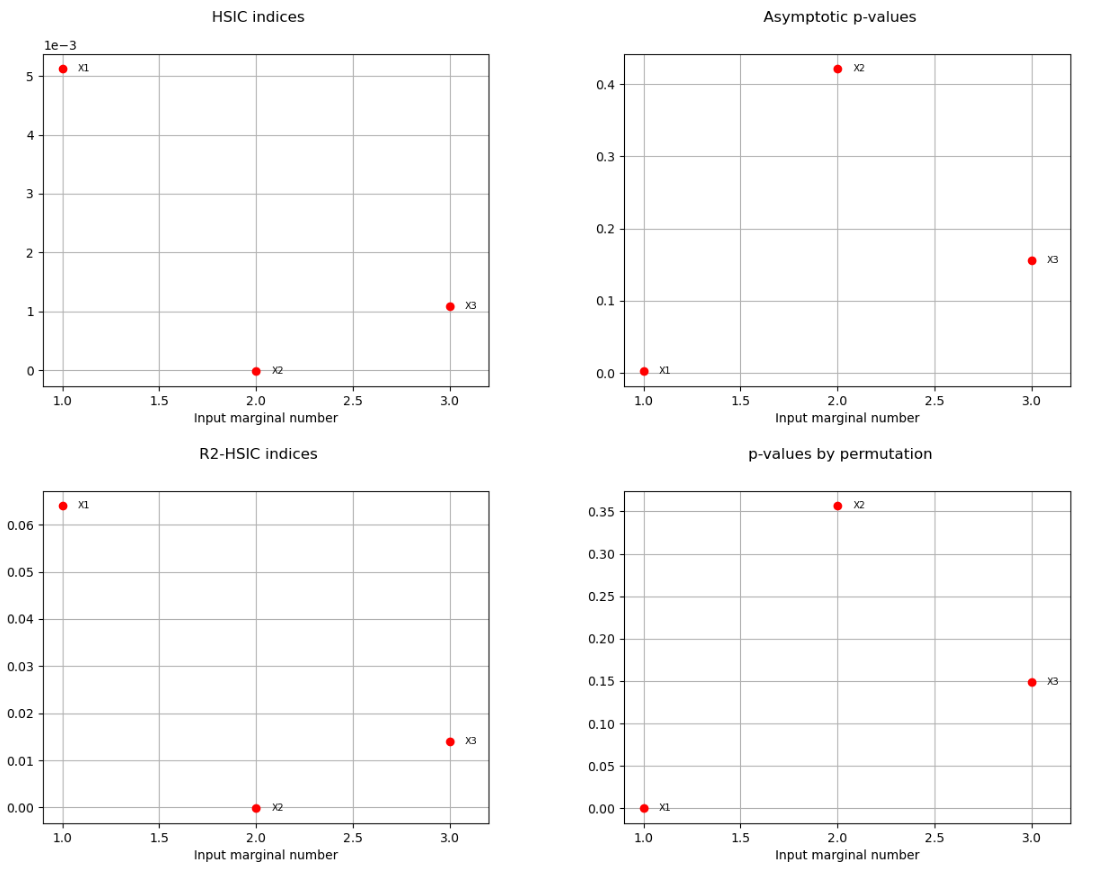
\includegraphics[width=0.65\textwidth]{figures/HSIC1.png}
% \end{figure}
% \end{frame}
% 
% 
% 
% 
% \begin{frame}[containsverbatim]	
% \frametitle{Example : Target sensitivity analysis on the Ishigami function}
% \begin{small}
% 
% \begin{lstlisting}
% estimatorType = ot.HSICVStat()
% 
% criticalDomain = ot.Interval(5, float('inf'))
% dist2criticalDomain = ot.DistanceToDomainFunction(criticalDomain)
% f = ot.SymbolicFunction(["x"], ["exp(-x)"])
% filterFunction = ot.ComposedFunction(f, dist2criticalDomain)
% 
% TSAEstimator = ot.HSICEstimatorTargetlSensitivity(
%     covarianceModelCollection, X, Y, estimatorType, 
%     filterFunction)
%     
% TSAEstimator.run()
% 
% graph1 = TSAEstimator.drawHSICIndices()
% graph2 = TSAEstimator.drawPValuesAsymptotic()
% graph3 = TSAEstimator.drawR2HSICIndices()
% graph4 = TSAEstimator.drawPValuesPermutation()
% \end{lstlisting}
% 
% \end{small}
% \end{frame}
% 
% \begin{frame}
% \frametitle{Example : Target sensitivity analysis on the Ishigami function}
% \begin{figure}
%    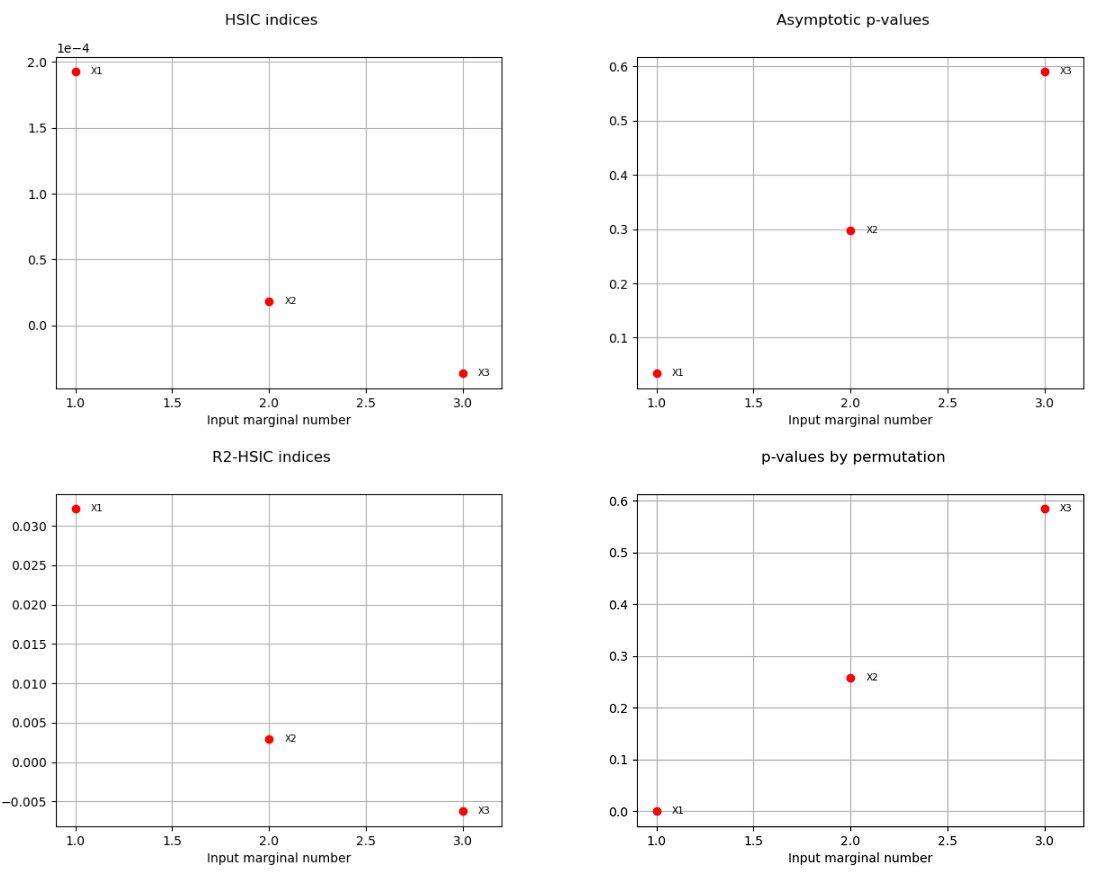
\includegraphics[width=0.65\textwidth]{figures/HSIC2.png}
% \end{figure}
% \end{frame}
% 
% \section{Metropolis-Hastings}
% % 
% \begin{frame}[containsverbatim]
% \frametitle{Metropolis-Hastings}
% 
% \begin{itemize}
% \item RandomWalkMH now updates with the instrumental in one go
% \item new Gibbs class that updates components sequentially
% \item Separate method to define the likelihood
% \item Handle improper prior via a log-pdf function
% \item Direct inconditional sampling according to a random variable
% \end{itemize}
% 
%  
% \begin{center}
% 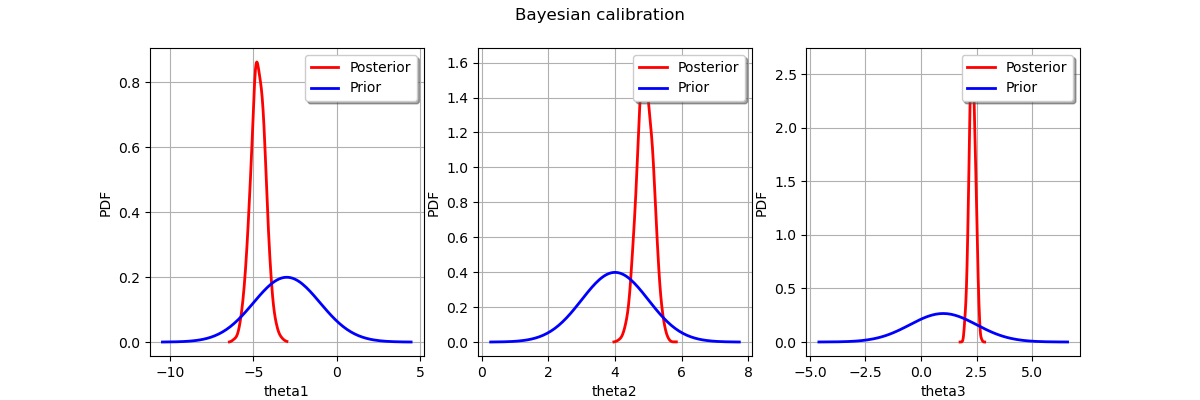
\includegraphics[width=0.9\textwidth]{figures/sphx_glr_plot_bayesian_calibration_002.png}
% \end{center}
% \end{frame}
% 
% \begin{frame}[containsverbatim]
% \frametitle{Metropolis-Hastings}
% 
% \lstset{language=python}
% \begin{lstlisting}
% from openturns import RandomWalkMetropolisHastings as RWMH
% rwmh1 = RWMH(prior, initialState, proposal1, [0])
% rwmh2 = RWMH(prior, initialState, proposal2, [1, 2])
% mh_coll = [rwmh1, rwmh2]
% for mh in mh_coll:
%     mh.setLikelihood(conditional, y_obs, linkFunction, x_obs)
% sampler = ot.Gibbs(mh_coll)
% x = sampler.getSample(1000)
% \end{lstlisting}
% 
% 
% \end{frame}
% 
% %%%%%%%%%%%%%%%%%%%%%%%%%%%%%%%%%%%%%%%%%%%%%%%%%%%%%%%%%%%%%%%%%%%%%%%%%%%%%
% \section{Iterative statistics}
% 
% %%%%%%%%%%%%%%%%%%%%%%%%%%%%%%%%%%%%%%%%%%%%%%%%%%%%%%%%%%%%%%%%%%%%%%%%%%%%%
% 
% \begin{frame}[containsverbatim]
% \frametitle{Iterative statistics}
% 
% \begin{itemize}
% \item Compute statistics without the need to store whole samples
% \item Moments / threshold exceedance / extrema
% \item Useful in HPC contexts
% \end{itemize}
% 
% \begin{center}
% 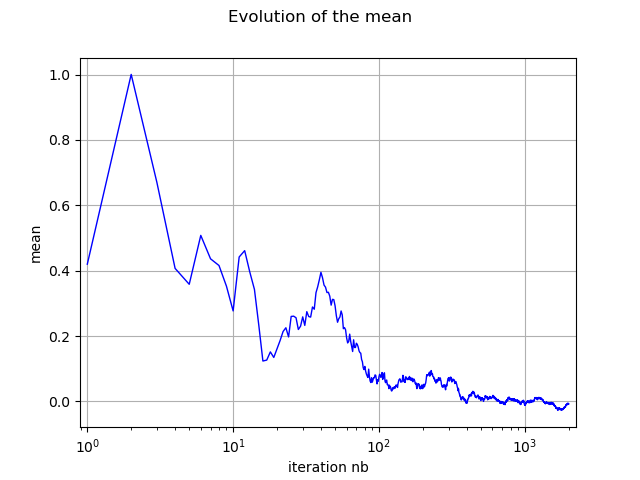
\includegraphics[width=0.5\textwidth]{figures/sphx_glr_plot_iterative_moments_001.png}
% \end{center}
% \end{frame}
% 
% \begin{frame}[containsverbatim]
% \frametitle{Iterative statistics}
% 
% \lstset{language=python}
% \begin{lstlisting}
% iter_mom = ot.IterativeMoments(order, dim)
% iter_ext = ot.IterativeExtrema(dim)
% iter_te = ot.IterativeThresholdExceedance(dim, 4.0)
% 
% for i in range(size):
%     x = rv.getRealization()
%     iter_mom.increment(x)
%     iter_ext.increment(x)
%     iter_te.increment(x)
% 
% xmin = iter_ext.getMin()
% xmax = iter_ext.getMax()
% variance = iter_mom.getVariance()
% skewness = iter_mom.getSkewness()
% pf = iter_te.getThresholdExceedance()
% \end{lstlisting}
% 
% 
% \end{frame}
% 
% %%%%%%%%%%%%%%%%%%%%%%%%%%%%%%%%%%%%%%%%%%%%%%%%%%%%%%%%%%%%%%%%%%%%%%%%%%%%%
% 
% \section{NAIS}
% 
% %%%%%%%%%%%%%%%%%%%%%%%%%%%%%%%%%%%%%%%%%%%%%%%%%%%%%%%%%%%%%%%%%%%%%%%%%%%%%
% 
% \begin{frame}[containsverbatim]
% \frametitle{NAIS}
% 
% \begin{itemize}
% \item Nonparametric Adaptive Importance Sampling (Morio 2015)
% 
% \item Adaptive method based on the idea of Importance Sampling
% 
% $$
% \widehat{P}^\text{IS}=\frac{1}{N} \sum_{i=1}^{N} {\mathbf{1}}_{g(\mathbf{x}_i)<T} \frac{h_0(\mathbf{x}_i)}{h(\mathbf{x}_i)}
% $$
% 
% \item Updates an importance density from KS (Gauss + Silverman)
% 
% \item Comparable to subset simulations
% 
% \item No tuning needed
% \end{itemize}
% 
% 
% \end{frame}
% 
% 
% 
% %%%%%%%%%%%%%%%%%%%%%%%%%%%%%%%%%%%%%%%%%%%%%%%%%%%%%%%%%%%%%%%%%%%%%%%%%%%%%
% \section{Galambos copula}
% 
% %%%%%%%%%%%%%%%%%%%%%%%%%%%%%%%%%%%%%%%%%%%%%%%%%%%%%%%%%%%%%%%%%%%%%%%%%%%%%
% 
% \begin{frame}
% \frametitle{Galambos copula}
% 
% \begin{itemize}
% \item bivariate extreme value copula
% $$ C(u_1, u_2) = u_1u_2\exp\left[(-\log(u_1))^{-\theta} + (-\log(u_2))^{-\theta}\right]^{-1/\theta} $$
% \item aims at modelling the dependence of rare events
% \end{itemize}
% 
% \begin{center}
% 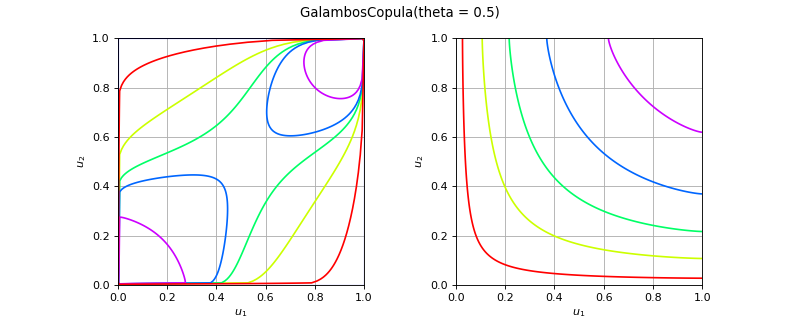
\includegraphics[width=0.8\textwidth]{figures/openturns-GalambosCopula-1.png}
% \end{center}
% 
% \end{frame}
% 
% %%%%%%%%%%%%%%%%%%%%%%%%%%%%%%%%%%%%%%%%%%%%%%%%%%%%%%%%%%%%%%%%%%%%%%%%%%%%%
% \section{Tensor product experiment}
% %%%%%%%%%%%%%%%%%%%%%%%%%%%%%%%%%%%%%%%%%%%%%%%%%%%%%%%%%%%%%%%%%%%%%%%%%%%%%
% 
% \begin{frame}[containsverbatim]
% \frametitle{Tensor product experiment}
% 
% \begin{itemize}
% \item Tensorize a set of elementary (d>=1) designs of experiments
% 
% $$
% \int_{\mathcal{X}} g(\boldsymbol{x}) f(\boldsymbol{x}) d\boldsymbol{x} 
%     \approx \sum_{i = 1}^{s_t} w_i g\left(\boldsymbol{x}_i\right)
% $$
% 
% \end{itemize}
% 
% 
% \begin{center}
% 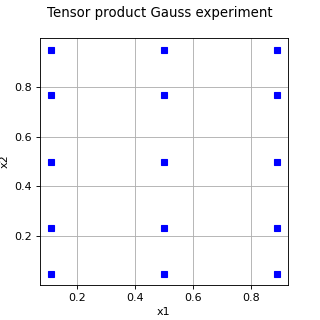
\includegraphics[width=0.38\textwidth]{figures/TensorProductExperiment.png}
% \end{center}
% \end{frame}
% 
% 
% \begin{frame}[containsverbatim]
% \frametitle{Tensor product experiment}
% 
% 
% \lstset{language=python}
% \begin{lstlisting}
% exp1 = ot.GaussProductExperiment(ot.Uniform(0.0, 1.0), [3])
% exp2 = ot.GaussProductExperiment(ot.Uniform(0.0, 1.0), [5])
% exp_tens = ot.TensorProductExperiment([exp1, exp2])
% nodes, weights = exp_tens.generateWithWeights()
% \end{lstlisting}
% 
% \end{frame}
% 
% %%%%%%%%%%%%%%%%%%%%%%%%%%%%%%%%%%%%%%%%%%%%%%%%%%%%%%%%%%%%%%%%%%%%%%%%%%%%%
% 
% \section{Multi-objective optimization}
% 
% \begin{frame}[containsverbatim]
% \frametitle{Multi-objective optimization}
% % \lstset{language=python}
% 
% % \begin{lstlisting}
% % 
% % \end{lstlisting}
% 
% \begin{itemize}
% \item massively parallel optimization Pagmo library from ESA
% \item 18 bio-inspired and evolutionary global algorithms
% \item 4 multi-objective algorithms
% \item some support batch evaluation / constraints / MINLP
% \end{itemize}
% 
% \begin{center}
% 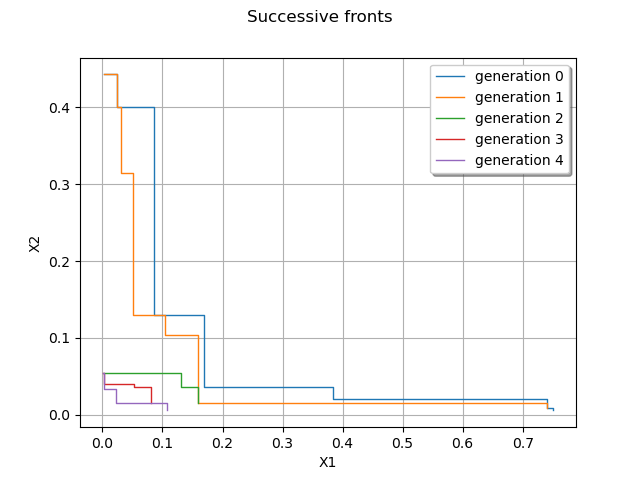
\includegraphics[width=0.4\textwidth]{figures/sphx_glr_plot_optimization_pagmo_002.png}
% \end{center}
% \end{frame}
% 
% 
% \begin{frame}[containsverbatim]
% \frametitle{Multi-objective optimization}
% 
% \lstset{language=python}
% \begin{lstlisting}
% pop0 = ot.ComposedDistribution([ot.Uniform(0.0, 1.0)] * 2).getSample(100)
% algo = ot.Pagmo(zdt1, 'nsga2', pop0)
% algo.setGenerationNumber(180)
% algo.run()
% result = algo.getResult()
% pop1 = result.getFinalPoints()
% fronts = result.getParetoFrontsIndices()
% \end{lstlisting}
% 
% 
% \end{frame}


%%%%%%%%%%%%%%%%%%%%%%%%%%%%%%%%%%%%%%%%%%%%%%%%%%%%%%%%%%%%%%%%%%%%%%%%%%%


\begin{frame}
\frametitle{Other improvements}

\begin{itemize}
\item Enabled Pagmo.moead_gen, Bonmin.Ecp/iFP optimization algorithms
\item ARM64 wheels for Apple silicon hardware
\item Continued bugfix / documentation / modules effort
\end{itemize}

\end{frame}

%%%%%%%%%%%%%%%%%%%%%%%%%%%%%%%%%%%%%%%%%%%%%%%%%%%%%%%%%%%%%%%%%%%%%%%%%%%%%

\begin{frame}
\frametitle{END}

Thank you for your attention!

Any questions?

\begin{center}

\includegraphics[width=0.2\textwidth]{figures/logo-ot-small}
\end{center}

\end{frame}

% %%%%%%%%%%%%%%%%%%%%%%%%%%%%%%%%%%%%%%%%%%%%%%%%%%%%%%%%%%%%%%%%%%%%%%%%%%%%%
% 
% \section{Bibliography}
% 
% \begin{frame}
% \frametitle{Bibliography}
% 
% \begin{itemize}
% \item Airbus, EDF, ONERA, Phimeca Engineering, IMACS.
% OpenTURNS, a scientific library usable as a Python module dedicated to the treatment of uncertainties, 
% \url{www.openturns.org}.
% \item Airbus, EDF, Phimeca Engineering, IMACS. Documentation of OpenTURNS, version 1.9. 
% \url{http://openturns.github.io/openturns/1.9/contents.html}
% \item  Michaël Baudin, Anne Dutfoy, Bertrand Iooss, and Anne-Laure Popelin. 
% OpenTURNS: An Industrial Software for Uncertainty Quantification in Simulation, 
% Handbook of Uncertainty Quantification, 
% pages 1-38. Springer International Publishing, 2016
% \end{itemize}
% 
% \end{frame}

\end{document}
